\documentclass{article}
\usepackage[utf8]{inputenc}
\usepackage[spanish]{babel}
\usepackage{listings}
\usepackage{graphicx}
\graphicspath{ {images/} }
\usepackage{cite}

\begin{document}

\begin{titlepage}
    \begin{center}
        \vspace*{1cm}
            
        \Huge
        \textbf{PROCESAMIENTO DE IMÁGENES  }
            
        \vspace{0.5cm}
        \LARGE
        Parcial 2
            
        \vspace{1.5cm}
            
        \textbf{Sergio Alberto Giraldo  Salazar \\ Diego Fernando Urbano Palma }
        
        \vfill
            
        \vspace{0.8cm}
            
        \Large
        Departamento de Ingeniería Electrónica y Telecomunicaciones\\
        Universidad de Antioquia\\
        Medellín\\
        Septiembre de 2021
            
    \end{center}
\end{titlepage}

\tableofcontents
\newpage
\section{Análisis del problema}\label{intro}
En el presente parcial se nos pide dar una interpretación de una imagen donde se submuestrea o se sobremuestrea para que sea compatible con la matriz de leds que se va montar en TINKERCAD.
Con el presente proyecto se evidencian  las siguientes dificultades, como lo serian la interpretación de datos por parte del TINKERCAD.\\
Otra dificultad para el proyecto es entender las matrices de datos que nos van a mostrar en el camino, como lo es la matriz RGB la cual nos dan el color de cada pixel para poder generar un código que nos  submuestre o sobremuestre la imagen. \\Saber que es sobremuestreo  y submuestre ya que es el eje de la practica 2 que en este momento estamos presentando. \\
Manejar correctamente las librerías de Arduino para darle el color deseado a nuestros leds mostrando la imagen después de haber completado el los procesos para tratar una imagen.


\section{funcionamiento del circuito} \label{contenido}

\begin{figure}[h]
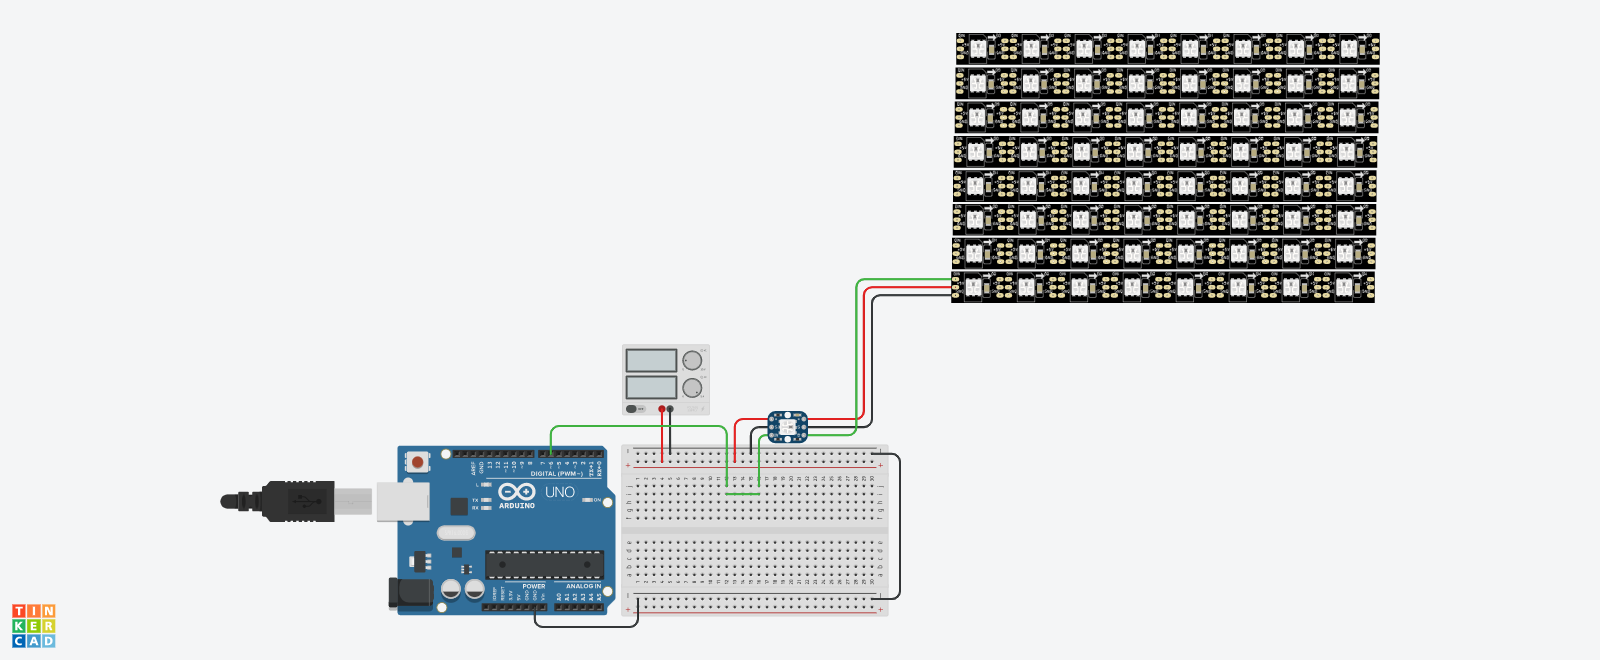
\includegraphics[width=10cm]{1.png}
\centering
\caption{Matriz de leds}
\label{fig:matriz de leds}
\end{figure}

\\
En la imagen se plantea una matriz de leds 8*8 donde el primer led a tomar en cuenta será el superior a la izquierda y de allí se ira avanzando hacia la derecha, decidimos tomar este orden para tener una mayor facilidad de compresión de como se ira reflejando los cambios en cada led.






\subsection{Citación}
Vamos a citar por ejemplo un artículo de \textbf{Albert Einstein} \cite{einstein}.
También es posible citar libros \cite{dirac} o documentos en línea \cite{knuthwebsite}.\\\\
Revisar en la última sección el formato de las referencias en IEEE.

\subsection{Incluir código en el documento}
%
A continuación, se presenta el código \ref{codigo_ejemplo}, que nos permite incluir en el informe partes de programa que requieran una explicación adicional.
\begin{lstlisting}[language=C++, label=codigo_ejemplo]
// Programa desarrollado, compilado y ejecutado en https://www.onlinegdb.com
#include <iostream>

/*
 * Esto es un comentario de varias lineas
 */

// Comentario de una sola linea

#define N 10

using namespace std;

int main()
{
    
    for( int i = 0 ; i < N ; i++ ){
        
        if( !(i % 2) )
            cout << " El valor de i es -> " << i << endl;
    }
    
    return 0;
}

//Resultado programa

/*
El valor de i es -> 0
El valor de i es -> 2
El valor de i es -> 4
El valor de i es -> 6
El valor de i es -> 8
*/
\end{lstlisting}
En la sección \ref{imagenes}, se presentará como añadir ilustraciones al texto.

\section{Inclusión de imágenes} \label{imagenes}

En la Figura (\ref{fig:cpplogo}), se presenta el logo de C++ contenido en la carpeta images.

\begin{figure}[h]
\includegraphics[width=4cm]{cpplogo.png}
\centering
\caption{Logo de C++}
\label{fig:cpplogo}
\end{figure}

Las secciones (\ref{intro}), (\ref{contenido}) y (\ref{imagenes}) dependen del estilo del documento.

\bibliographystyle{IEEEtran}
\bibliography{references}

\end{document}
